
\chapter{Design to analyze existing system}

  The following sections describe the set of questions that we aspire to answer and what are the experimental configurations, setup and 
metrics used to answer the same. 

  \section{Experimental scenarios}
    
    Before we try to establish the questions that we wish to answer, we list the set of different scenarios in which a containers in a 
system can exist based on which we try to frame questions. The following are the possible experimental scenarios under which memory 
pressure maybe generated that triggers reclamation. And our main focus would be to understand how memory pressure would affect applications 
in these scenarios,

    \begin{enumerate}
      \item All containers exceed: All containers are above soft limits
      \item None of the containers exceed: All containers are below soft limits or have no soft limits
      \item Few containers exceed and the rest don't
    \end{enumerate}
  
  \section{Questions of interest}
    \label{section_questions}
  
    The following are the list of questions of interest in each of the above described scenarios,
    
    \subsection{All containers exceed}
      
      \begin{enumerate}
	\item Is SMR purely based on exceed value of the container ?
	\item Does only SMR occur when containers are exceeding ? if not, how much of memory is reclaimed using GLR ?  In what ratio does 
SMR and GLR vary based on system memory pressure ?
	\item How much of memory is reclaimed from a container in a single reclamation request ?
	\item In what ratio does SMR and GLR vary based on container soft limits ?
	%\item How is memory reassigned to containers when system pressure reduces ?
	
	\item Does setting containers with higher memory limits using existing memory reservations always guarantee higher priority to a 
one container over the other while reclamation ?
	\item When containers are exceeding by the same values, in what order and how much of memory reclamation occurs from different 
containers ?
	\item When containers are exceeding by the different values, in what order and how much of memory reclamation occurs from different 
containers ?
      \end{enumerate}
  
  \subsection{None of the containers exceed}
  
    \begin{enumerate}
      \item Does our hypotheses of reclamation below soft limits falling back to native system reclamation hold good ?
      \item Both containers not exceeding / containers without soft limits behave similarly ? 
    \end{enumerate}
  
  \subsection{A few containers exceed, but the others do not}
  
    \begin{enumerate}
      \item Is the soft limit that is assigned to a container a definite guarantee ? If not, what role does it play in memory reclamation ?
      \item How is memory is reclaimed from the containers that exceed and the containers that don’t ? Which of the two are more penalized ?
    \end{enumerate}
  
  \section{Experimental guidelines}
    \label{section_guidelines}
    
    The following are a set of guidelines that any empirical analysis of memory management techniques in a container environment must 
abide by.  All experiments presented in this report were designed and executed around these guidelines.

    \begin{enumerate}
      \item All experiments must comprise of a set of valid configurations that could be readily applied to any container based OS-level 
virtualization environment. These configurations must be readily available, and easy to apply.
      \item Set of workloads used must always be configured in such a way that it is memory intensive, and always throttles only on memory 
and no other resource.
      \item All experiments must be reproducible and statistically correct.      
    \end{enumerate}

  \section{Experimental configurations}
    
    As pointed out in section \ref{section_guidelines}, the set of configurations used for an analysis of memory management techniques in a 
container environment must be relevant, and easy to apply. The following configurations fit this criteria, and have been used for the 
evaluation.
    
    \begin{itemize}
      \item \textbf{Number of containers:} The number of containers that are currently executing in the system.
      \item \textbf{Memory soft limit of container:} The minimum promised memory to a given container by the system on which the 
container is executing.
      \item \textbf{Memory hard limit of container:} The maximum memory that can be assigned to a container by the system on which the 
container is executing.
      \item \textbf{Memory usage of each container:} The usage of a container at a given point in time, that is generated by the workload 
executing inside the container.
      \item \textbf{Workload:} The workload that is running inside each of the container. Workloads can vary based on the type of operation 
they perform, the ratio of anonymous memory pages they consume to that of page cache pages.  
      \item \textbf{External memory pressure:} The memory pressure that is generated in the system in order to reduce the free memory 
available in the system and trigger memory reclamation. This pressure could be either generated by a process on the same system / driver 
that is running in the host system.
      \item \textbf{Size of machine:} Size of Machine refers to the maximum memory available in the system inside which all the 
containers are executing.      
    \end{itemize}  
  
  \section{Metrics of interest}
  
    The following are the metrics of interest to us that would help us analyze the experiments.
      
	\begin{enumerate}
	 \item \textbf{Memory assigned to each container:} Total memory assigned to a container at any given instant
	 \item \textbf{Soft memory reclaimed for each container:} Memory reclaimed from each container using SMR
	 \item \textbf{Total memory reclaimed for each container:} Total Memory reclaimed from container (SMR + GLR)
	 \item \textbf{Memory reclaimed using GLR:} Memory reclaimed from all containers and other processes running on system using GLR
	 \item \textbf{Memory reassigned for each container:} Memory reassigned to each container on freeing up of memory
	 \item \textbf{Application specific metrics:} Application metrics of the workload running inside containers like throughput, total 
time taken etc.
	\end{enumerate}
  
  \section{Workloads}
  
    This section presents the list of workloads that we have used as primary candidates to evaluate our empirical evaluations. All 
workloads are chosen keeping in mind the memory intensive nature as mentioned in \ref{section_guidelines}.  
    
    \subsection{Synthetic workloads}
    
      These are the list of Synthetic workloads we have used to establish our problem.
      
      \subsubsection{Stress}
	Stress \cite{stress} is a deliberately simple workload generator for POSIX systems. It imposes a configurable amount of CPU, 
memory, I/O, and disk stress on the system. It is written in C and has been developed by people at Harvard university. 
      
      \subsubsection{Memory hogger}
	Memory Hogger is a simple C program that allocates an array of specified memory using a simple \texttt{malloc()} and repeatedly 
writes to these array locations. This only consumes anonymous memory pages.
      
      \subsubsection{File hogger}
	File Hogger is a simple python program that creates a file with specified size and repeatedly updates it line by line there by 
consuming both anonymous pages and file backed pages.

    \subsection{Real workloads}
    
      These are the list of real workloads we have used to show how the existing problems affect real work applications.
      
      \subsubsection{MongoDB}
	MongoDB \cite{Mongodb} is an open-source, document database designed for ease of development and scaling. Classified as a NoSQL 
database program, MongoDB avoids the traditional table-based relational database structure in favor of JSON-like documents with dynamic 
schema. It follows a memory hungry approach where it tries to use up most of system and it actually leaves it up to the OS's VMM to tell it 
to release the memory.

      \subsubsection{Redis}
	Redis \cite{Redis} is a in-memory data structure store, used as database, cache and message broker. It is used to store a large 
number of in-memory key-value pairs. Its in-memory nature makes it a prime candidate to use it as a workload in our empirical evaluations.
   
    \subsection{YCSB benchmark}
	We use YCSB \cite{cooper2010benchmarking} (Yahoo Cloud Server Benchmark) project as the benchmark to generate the clients evaluate 
to the performance of our real workloads i.e MongoDB and Redis servers. The goal of YSCB is to develop performance comparisons of the new 
generation of cloud data serving systems. It is a framework and common set of workloads for evaluating the performance of different 
“key-value” stores.

  \section{Experimental setup}
  
    The following section describes the experimental setups used. There were two experimental setups used.  The second setup which involved 
a derivative cloud setup was used to establish the problem in the derivative cloud setup using Real workloads.
    
    \subsection{Native container testbed}
      \label{section_testbed_native}
      
      \begin{figure}
	\centering
	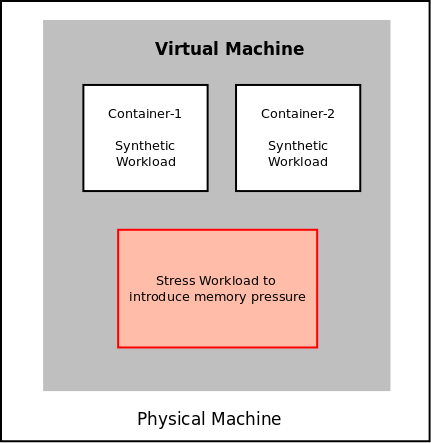
\includegraphics[width=0.5\textwidth]{images/native_setup.png}
	\caption{Native container testbed}
	\label{img_native_setup}
      \end{figure}
      
       The native testbed consisted of running containers inside a host machine (running inside VM in our case) in complete isolation from 
the external environment as shown in Fig:\ref{img_derived_setup}. This setup which involved a native container testbed, was used to 
understand the existing memory reclamations and establish the problem in a native system using \textbf{synthetic workloads}.
	
      \subsubsection{Host}
	
	\begin{enumerate}
	  \item Intel Core i5-4430 processor @ 3.00GHz
	  \item 4 cores of CPU (with hyper threading support)
	  \item 1 TB of hard disk space
	  \item 8 GB RAM
	  \item Ubuntu 14.04 LTS desktop, 64 bit 
	  \item Kernel version 4.5
	  \item KVM Hypervisor
	\end{enumerate}
      
      \subsubsection{Guest}
	
	\begin{enumerate}
	  \item 3 cores of CPU (with hyper threading support)
	  \item 20 GB of virtual disk space
	  \item 2-6 GB RAM (based on experimental configuration)
	  \item Ubuntu 16.04 LTS desktop, 64 bit
	  \item Kernel version 4.7
	\end{enumerate}
	
      \subsubsection{Workloads used}
	
	Memory Hogger and File Hogger was used to generate the memory pressure inside the containers. External pressure was generated 
using Stress workload running directly on the host machine.

      \subsubsection{Experimental flow}
	
	Most experiments involved setting up of 2 containers. Workloads were used to introduce system memory pressure from containers. At 
this point there was no memory pressure in the system (free memory was still available). Now the external pressure using Stress was 
introduced after about 20s which created memory pressure in the system that triggered reclamation. The external pressure kept on increasing 
by 200 MB in intervals of 40s. Each interval had a gap of 10s for memory to be reassigned to containers.

    \subsection{Derivative cloud testbed}
      \label{section_testbed_derivative}
      
       The derivative cloud testbed consisted of running server containers inside a virtual machine (VM-1) which was running on top of a 
physical host machine. Another virtual machine (VM-2) was used to generate clients who connected to servers containers running inside VM-1 
as shown in Fig:\ref{img_derived_setup}. This setup was used to understand the impact of existing memory reclamation patterns on real 
workloads running on a derivative cloud setting.
      
      \begin{figure}
	\centering
	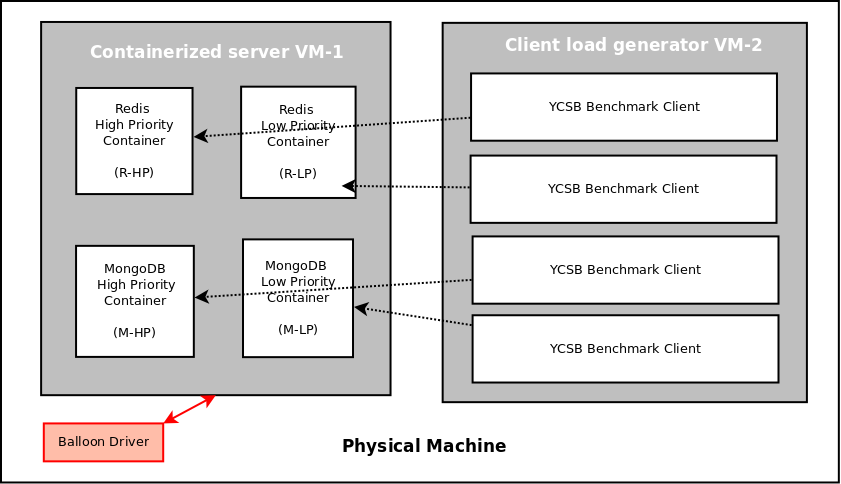
\includegraphics[width=1\textwidth]{images/Experimental_Setup.png}
	\caption{Derivative cloud testbed}
	\label{img_derived_setup}
      \end{figure}
      
      \subsubsection{Host}
	
	\begin{enumerate}
	  \item Intel Xeon E5507 @ 2.27GHz
	  \item 8 cores of CPU (with hyper-threading support)
	  \item 125 GB of attached storage, Unlimited NFS attached storage 
	  \item 24 GB RAM
	  \item Ubuntu 14.04 LTS server, 64 bit 
	  \item Kernel version 3.13
	  \item KVM Hypervisor with memory ballooning enabled
	  \item Guest machines were connected using a software bridge
	\end{enumerate}
      
      \subsubsection{Guest}
	
	The two VMs used in this setup are described here.
	
	\noindent \textbf{VM-1:} Running server containers
	\begin{enumerate}
	  \item 6 cores of pinned CPUs (with hyper threading support)
	  \item 175 GB of virtual disk space (Storage was provisioned using NFS)
	  \item 16 GB RAM
	  \item Ubuntu 16.04 LTS desktop, 64 bit
	  \item Kernel version 4.7
	  \item Containers inside guest were multiplexed using NAT forwarding
	\end{enumerate}
	
	\noindent \textbf{VM-2:} Running clients that connect to server containers
	\begin{enumerate}
	  \item 1 core of pinned CPU (with hyper threading support)
	  \item 20 GB of virtual disk space (Storage was provisioned using NFS)
	  \item 6 GB RAM
	  \item Ubuntu 16.04 LTS desktop, 64 bit
	  \item Kernel version 4.7
	\end{enumerate}
	
      \subsubsection{Workloads used}
	
	Redis and MongoDB was used to generate the memory pressure inside the containers. External pressure was generated by varying guest 
balloon size triggered from the host.

      \subsubsection{Experimental flow}
	
	Most experiments involved setting up of 4 containers (2 Redis containers and 2 MongoDB containers). Workloads were used to 
introduce system memory pressure from containers. At this point there was no memory pressure in the system (free memory was still 
available). Now the external pressure was introduced by reducing the guest VM size after 100s, which in turn trigger memory reclamation at 
the guest VM.
	